
\documentclass[11pt]{article}
\usepackage[%
  papersize={12.8cm,9.6cm},
  hmargin=1cm,%
  vmargin=1cm,%
  head=0.4cm,% might be changed later
  headsep=0pt,%
  foot=0.5cm% might be changed later
]{geometry}% http://ctan.org/pkg/geometry

\RequirePackage{amsmath}
\RequirePackage{amssymb}
\RequirePackage{amsthm}
%\RequirePackage{algorithmic}
%\RequirePackage{algorithm}
%\RequirePackage{theorem}
%\RequirePackage{eucal}
\RequirePackage{color}
\RequirePackage{url}
\RequirePackage{mdwlist}

\RequirePackage[all]{xy}
\CompileMatrices
\RequirePackage{hyperref}
\RequirePackage{graphicx}
\RequirePackage{relsize}


% xelatex:
\usepackage{fontspec}
\defaultfontfeatures{Ligatures=TeX}
%\usepackage[small,sf,bf]{titlesec}
%\setromanfont{DejaVu Serif}
%\setromanfont{Droid Serif}
%\setromanfont{Gentium} % nice! a bit fluffy
\setromanfont{Gentium Book Basic} % more bold



\RequirePackage{graphicx}
\usepackage{color}
\usepackage{amsfonts}


%\def\heading #1{\vskip 20pt \noindent\underline{\large \bf #1}\vskip 5pt}
\def\heading #1{\centerline{\underline{\bf\LARGE #1}}}
\def\vsp {\vskip 0.5cm}

\def\ket #1{|#1\rangle}
%\def\point {\vskip 5pt $\to$\ \ }
%\def\point {\vskip 5pt $\Longrightarrow$\ \ }
%\def\point {\vskip 5pt $\bigodot$\ \ }
\def\point {\vskip 5pt $\hookrightarrow$\ \ }

\begin{document}

\large

\pagenumbering{gobble}

%%%%%%%%%%%%%%%%%%%%%%%%%%%%%%%%%%%%%%%%%%%%%%%%%%%%%%%%%%%


\centerline{\LARGE }
\vskip 0.5cm
\centerline{\LARGE Distributivity, size, homomorphism}
\vskip 0.5cm
\centerline{\LARGE }

\vskip 1cm

\centerline{\Large Simon Burton}

\vskip 0.5cm

\centerline{School of Physics, The University of Sydney}


%\newpage %%%%%%%%%%%%%%%%%%%%%%%%%%%%%%%%%%%%%%%%%%%%%%%%%%
%
%\begin{center}
%\includegraphics[width=0.2\textwidth]{ExclamationMark.pdf}
%\end{center}
%
%\vskip 0.5cm
%\hspace{4 em} Possible \hspace{9 em} Actual
%

\newpage %%%%%%%%%%%%%%%%%%%%%%%%%%%%%%%%%%%%%%%%%%%%%%%%%%

\heading{Matrix multiplication}

\centerline{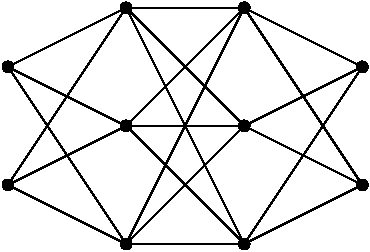
\includegraphics[]{pic-trellis.pdf}}

Distributivity:
$$
    a(b + c) = ab + ac
$$
\vsp\vsp
\vsp\vsp

\newpage %%%%%%%%%%%%%%%%%%%%%%%%%%%%%%%%%%%%%%%%%%%%%%%%%%

\heading{Minimum weight path}
\centerline{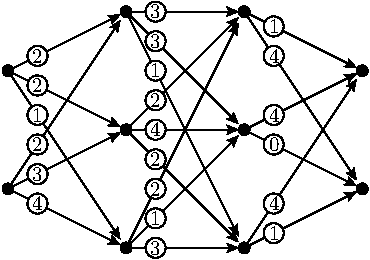
\includegraphics[]{pic-minpath-0.pdf}}
$$
    |\mbox{paths}| = 2.3.3.2 = 36
$$

\newpage %%%%%%%%%%%%%%%%%%%%%%%%%%%%%%%%%%%%%%%%%%%%%%%%%%

\heading{Minimum weight path}
\centerline{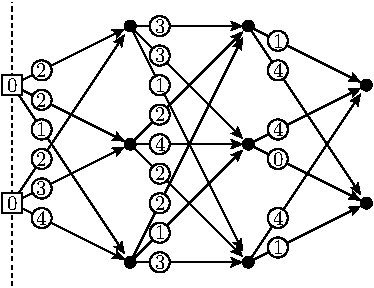
\includegraphics[]{pic-minpath-1.pdf}}

\newpage %%%%%%%%%%%%%%%%%%%%%%%%%%%%%%%%%%%%%%%%%%%%%%%%%%

\heading{Minimum weight path}
\centerline{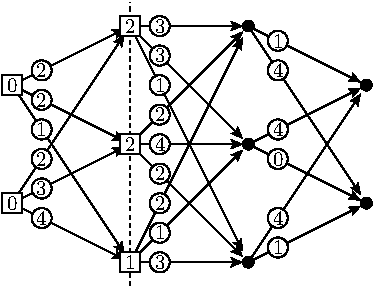
\includegraphics[]{pic-minpath-2.pdf}}

\newpage %%%%%%%%%%%%%%%%%%%%%%%%%%%%%%%%%%%%%%%%%%%%%%%%%%

\heading{Minimum weight path}
\centerline{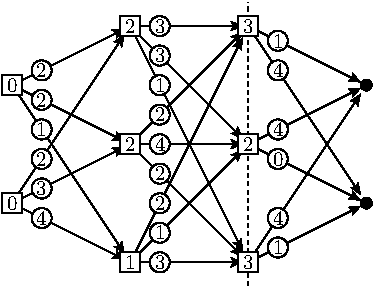
\includegraphics[]{pic-minpath-3.pdf}}

\newpage %%%%%%%%%%%%%%%%%%%%%%%%%%%%%%%%%%%%%%%%%%%%%%%%%%

\heading{Minimum weight path}
\centerline{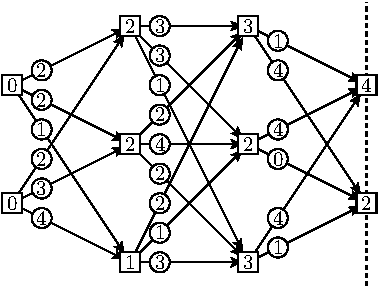
\includegraphics[]{pic-minpath-4.pdf}}

Distributivity:
$$
    a + \min(b, c) = \min(a+b, a+c)
$$


\newpage %%%%%%%%%%%%%%%%%%%%%%%%%%%%%%%%%%%%%%%%%%%%%%%%%%

\heading{Linear recurrence relations}

\vsp
\centerline{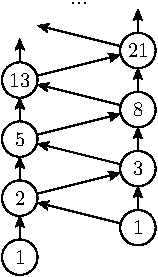
\includegraphics[]{pic-fibonacci.pdf}}
$$
    a_{n+2} = a_{n+1} + a_n
$$



\newpage %%%%%%%%%%%%%%%%%%%%%%%%%%%%%%%%%%%%%%%%%%%%%%%%%%

\heading{Linear recurrence relations}

\vsp
\centerline{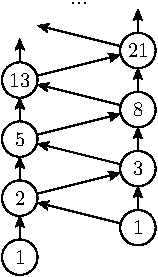
\includegraphics[]{pic-fibonacci.pdf}}
$$
    Sn := n+1
$$
$$
    f(SSn) = f(Sn) + f(n).
$$



\newpage %%%%%%%%%%%%%%%%%%%%%%%%%%%%%%%%%%%%%%%%%%%%%%%%%%


\end{document} %%%%%%%%%%%%%%%%%%%%%%%%%%%%%%%%%%%%%%%%%%%%%%%%%%%%%%%%%%%

